\documentclass[1p]{elsarticle_modified}
%\bibliographystyle{elsarticle-num}

%\usepackage[colorlinks]{hyperref}
%\usepackage{abbrmath_seonhwa} %\Abb, \Ascr, \Acal ,\Abf, \Afrak
\usepackage{amsfonts}
\usepackage{amssymb}
\usepackage{amsmath}
\usepackage{amsthm}
\usepackage{scalefnt}
\usepackage{amsbsy}
\usepackage{kotex}
\usepackage{caption}
\usepackage{subfig}
\usepackage{color}
\usepackage{graphicx}
\usepackage{xcolor} %% white, black, red, green, blue, cyan, magenta, yellow
\usepackage{float}
\usepackage{setspace}
\usepackage{hyperref}

\usepackage{tikz}
\usetikzlibrary{arrows}

\usepackage{multirow}
\usepackage{array} % fixed length table
\usepackage{hhline}

%%%%%%%%%%%%%%%%%%%%%
\makeatletter
\renewcommand*\env@matrix[1][\arraystretch]{%
	\edef\arraystretch{#1}%
	\hskip -\arraycolsep
	\let\@ifnextchar\new@ifnextchar
	\array{*\c@MaxMatrixCols c}}
\makeatother %https://tex.stackexchange.com/questions/14071/how-can-i-increase-the-line-spacing-in-a-matrix
%%%%%%%%%%%%%%%

\usepackage[normalem]{ulem}

\newcommand{\msout}[1]{\ifmmode\text{\sout{\ensuremath{#1}}}\else\sout{#1}\fi}
%SOURCE: \msout is \stkout macro in https://tex.stackexchange.com/questions/20609/strikeout-in-math-mode

\newcommand{\cancel}[1]{
	\ifmmode
	{\color{red}\msout{#1}}
	\else
	{\color{red}\sout{#1}}
	\fi
}

\newcommand{\add}[1]{
	{\color{blue}\uwave{#1}}
}

\newcommand{\replace}[2]{
	\ifmmode
	{\color{red}\msout{#1}}{\color{blue}\uwave{#2}}
	\else
	{\color{red}\sout{#1}}{\color{blue}\uwave{#2}}
	\fi
}

\newcommand{\Sol}{\mathcal{S}} %segment
\newcommand{\D}{D} %diagram
\newcommand{\A}{\mathcal{A}} %arc


%%%%%%%%%%%%%%%%%%%%%%%%%%%%%5 test

\def\sl{\operatorname{\textup{SL}}(2,\Cbb)}
\def\psl{\operatorname{\textup{PSL}}(2,\Cbb)}
\def\quan{\mkern 1mu \triangleright \mkern 1mu}

\theoremstyle{definition}
\newtheorem{thm}{Theorem}[section]
\newtheorem{prop}[thm]{Proposition}
\newtheorem{lem}[thm]{Lemma}
\newtheorem{ques}[thm]{Question}
\newtheorem{cor}[thm]{Corollary}
\newtheorem{defn}[thm]{Definition}
\newtheorem{exam}[thm]{Example}
\newtheorem{rmk}[thm]{Remark}
\newtheorem{alg}[thm]{Algorithm}

\newcommand{\I}{\sqrt{-1}}
\begin{document}

%\begin{frontmatter}
%
%\title{Boundary parabolic representations of knots up to 8 crossings}
%
%%% Group authors per affiliation:
%\author{Yunhi Cho} 
%\address{Department of Mathematics, University of Seoul, Seoul, Korea}
%\ead{yhcho@uos.ac.kr}
%
%
%\author{Seonhwa Kim} %\fnref{s_kim}}
%\address{Center for Geometry and Physics, Institute for Basic Science, Pohang, 37673, Korea}
%\ead{ryeona17@ibs.re.kr}
%
%\author{Hyuk Kim}
%\address{Department of Mathematical Sciences, Seoul National University, Seoul 08826, Korea}
%\ead{hyukkim@snu.ac.kr}
%
%\author{Seokbeom Yoon}
%\address{Department of Mathematical Sciences, Seoul National University, Seoul, 08826,  Korea}
%\ead{sbyoon15@snu.ac.kr}
%
%\begin{abstract}
%We find all boundary parabolic representation of knots up to 8 crossings.
%
%\end{abstract}
%\begin{keyword}
%    \MSC[2010] 57M25 
%\end{keyword}
%
%\end{frontmatter}

%\linenumbers
%\tableofcontents
%
\newcommand\colored[1]{\textcolor{white}{\rule[-0.35ex]{0.8em}{1.4ex}}\kern-0.8em\color{red} #1}%
%\newcommand\colored[1]{\textcolor{white}{ #1}\kern-2.17ex	\textcolor{white}{ #1}\kern-1.81ex	\textcolor{white}{ #1}\kern-2.15ex\color{red}#1	}

{\Large $\underline{12a_{0677}~(K12a_{0677})}$}

\setlength{\tabcolsep}{10pt}
\renewcommand{\arraystretch}{1.6}
\vspace{1cm}\begin{tabular}{m{100pt}>{\centering\arraybackslash}m{274pt}}
\multirow{5}{120pt}{
	\centering
	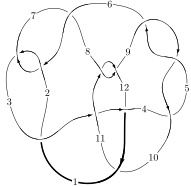
\includegraphics[width=112pt]{../../../GIT/diagram.site/Diagrams/png/1478_12a_0677.png}\\
\ \ \ A knot diagram\footnotemark}&
\allowdisplaybreaks
\textbf{Linearized knot diagam} \\
\cline{2-2}
 &
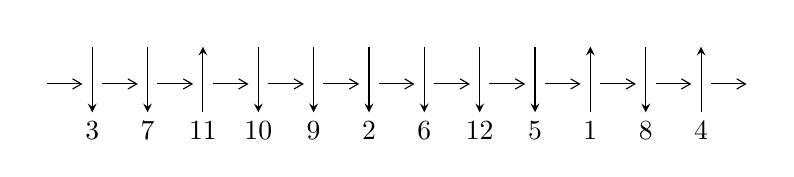
\begin{tikzpicture}[x=20pt, y=17pt]
	% nodes
	\node (C0) at (0, 0) {};
	\node (C1) at (1, 0) {};
	\node (C1U) at (1, +1) {};
	\node (C1D) at (1, -1) {3};

	\node (C2) at (2, 0) {};
	\node (C2U) at (2, +1) {};
	\node (C2D) at (2, -1) {7};

	\node (C3) at (3, 0) {};
	\node (C3U) at (3, +1) {};
	\node (C3D) at (3, -1) {11};

	\node (C4) at (4, 0) {};
	\node (C4U) at (4, +1) {};
	\node (C4D) at (4, -1) {10};

	\node (C5) at (5, 0) {};
	\node (C5U) at (5, +1) {};
	\node (C5D) at (5, -1) {9};

	\node (C6) at (6, 0) {};
	\node (C6U) at (6, +1) {};
	\node (C6D) at (6, -1) {2};

	\node (C7) at (7, 0) {};
	\node (C7U) at (7, +1) {};
	\node (C7D) at (7, -1) {6};

	\node (C8) at (8, 0) {};
	\node (C8U) at (8, +1) {};
	\node (C8D) at (8, -1) {12};

	\node (C9) at (9, 0) {};
	\node (C9U) at (9, +1) {};
	\node (C9D) at (9, -1) {5};

	\node (C10) at (10, 0) {};
	\node (C10U) at (10, +1) {};
	\node (C10D) at (10, -1) {1};

	\node (C11) at (11, 0) {};
	\node (C11U) at (11, +1) {};
	\node (C11D) at (11, -1) {8};

	\node (C12) at (12, 0) {};
	\node (C12U) at (12, +1) {};
	\node (C12D) at (12, -1) {4};
	\node (C13) at (13, 0) {};

	% arrows
	\draw[->,>={angle 60}]
	(C0) edge (C1) (C1) edge (C2) (C2) edge (C3) (C3) edge (C4) (C4) edge (C5) (C5) edge (C6) (C6) edge (C7) (C7) edge (C8) (C8) edge (C9) (C9) edge (C10) (C10) edge (C11) (C11) edge (C12) (C12) edge (C13) ;	\draw[->,>=stealth]
	(C1U) edge (C1D) (C2U) edge (C2D) (C3D) edge (C3U) (C4U) edge (C4D) (C5U) edge (C5D) (C6U) edge (C6D) (C7U) edge (C7D) (C8U) edge (C8D) (C9U) edge (C9D) (C10D) edge (C10U) (C11U) edge (C11D) (C12D) edge (C12U) ;
	\end{tikzpicture} \\
\hhline{~~} \\& 
\textbf{Solving Sequence} \\ \cline{2-2} 
 &
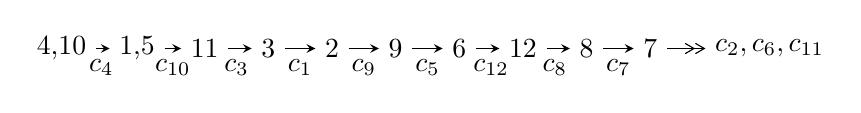
\begin{tikzpicture}[x=23pt, y=7pt]
	% node
	\node (A0) at (-1/8, 0) {4,10};
	\node (A1) at (17/16, 0) {1,5};
	\node (A2) at (17/8, 0) {11};
	\node (A3) at (25/8, 0) {3};
	\node (A4) at (33/8, 0) {2};
	\node (A5) at (41/8, 0) {9};
	\node (A6) at (49/8, 0) {6};
	\node (A7) at (57/8, 0) {12};
	\node (A8) at (65/8, 0) {8};
	\node (A9) at (73/8, 0) {7};
	\node (C1) at (1/2, -1) {$c_{4}$};
	\node (C2) at (13/8, -1) {$c_{10}$};
	\node (C3) at (21/8, -1) {$c_{3}$};
	\node (C4) at (29/8, -1) {$c_{1}$};
	\node (C5) at (37/8, -1) {$c_{9}$};
	\node (C6) at (45/8, -1) {$c_{5}$};
	\node (C7) at (53/8, -1) {$c_{12}$};
	\node (C8) at (61/8, -1) {$c_{8}$};
	\node (C9) at (69/8, -1) {$c_{7}$};
	\node (A10) at (11, 0) {$c_{2},c_{6},c_{11}$};

	% edge
	\draw[->,>=stealth]	
	(A0) edge (A1) (A1) edge (A2) (A2) edge (A3) (A3) edge (A4) (A4) edge (A5) (A5) edge (A6) (A6) edge (A7) (A7) edge (A8) (A8) edge (A9) ;
	\draw[->>,>={angle 60}]	
	(A9) edge (A10);
\end{tikzpicture} \\ 

\end{tabular} \\

\footnotetext{
The image of knot diagram is generated by the software ``\textbf{Draw programme}" developed by Andrew Bartholomew(\url{http://www.layer8.co.uk/maths/draw/index.htm\#Running-draw}), where we modified some parts for our purpose(\url{https://github.com/CATsTAILs/LinksPainter}).
}\phantom \\ \newline 
\centering \textbf{Ideals for irreducible components\footnotemark of $X_{\text{par}}$} 
 
\begin{align*}
I^u_{1}&=\langle 
-1.64622\times10^{208} u^{95}-1.80313\times10^{208} u^{94}+\cdots+1.14976\times10^{209} b+3.29451\times10^{209},\\
\phantom{I^u_{1}}&\phantom{= \langle  }-1.64003\times10^{210} u^{95}-3.12587\times10^{210} u^{94}+\cdots+1.14976\times10^{209} a+1.12635\times10^{211},\\
\phantom{I^u_{1}}&\phantom{= \langle  }u^{96}+2 u^{95}+\cdots-44 u-1\rangle \\
I^u_{2}&=\langle 
- u^{23}+u^{22}+\cdots+b+1,\;u^{23}- u^{22}+\cdots+a-2 u,\;u^{24}- u^{23}+\cdots-2 u-1\rangle \\
I^u_{3}&=\langle 
b- u,\;a- u,\;u^{15}+3 u^{13}+u^{10}-5 u^9+2 u^8- u^6+5 u^5-2 u^4+u^3+u^2-2 u+1\rangle \\
\\
\end{align*}
\raggedright * 3 irreducible components of $\dim_{\mathbb{C}}=0$, with total 135 representations.\\
\footnotetext{All coefficients of polynomials are rational numbers. But the coefficients are sometimes approximated in decimal forms when there is not enough margin.}
\newpage
\renewcommand{\arraystretch}{1}
\centering \section*{I. $I^u_{1}= \langle -1.65\times10^{208} u^{95}-1.80\times10^{208} u^{94}+\cdots+1.15\times10^{209} b+3.29\times10^{209},\;-1.64\times10^{210} u^{95}-3.13\times10^{210} u^{94}+\cdots+1.15\times10^{209} a+1.13\times10^{211},\;u^{96}+2 u^{95}+\cdots-44 u-1 \rangle$}
\flushleft \textbf{(i) Arc colorings}\\
\begin{tabular}{m{7pt} m{180pt} m{7pt} m{180pt} }
\flushright $a_{4}=$&$\begin{pmatrix}1\\0\end{pmatrix}$ \\
\flushright $a_{10}=$&$\begin{pmatrix}0\\u\end{pmatrix}$ \\
\flushright $a_{1}=$&$\begin{pmatrix}14.2640 u^{95}+27.1870 u^{94}+\cdots-4367.63 u-97.9634\\0.143179 u^{95}+0.156826 u^{94}+\cdots-29.3497 u-2.86538\end{pmatrix}$ \\
\flushright $a_{5}=$&$\begin{pmatrix}1\\u^2\end{pmatrix}$ \\
\flushright $a_{11}=$&$\begin{pmatrix}-20.9593 u^{95}-40.0137 u^{94}+\cdots+6954.20 u+166.245\\-1.49859 u^{95}-2.89068 u^{94}+\cdots+755.253 u+25.2178\end{pmatrix}$ \\
\flushright $a_{3}=$&$\begin{pmatrix}47.3979 u^{95}+92.0448 u^{94}+\cdots-21779.0 u-745.556\\-1.33998 u^{95}-2.62161 u^{94}+\cdots+518.832 u+13.9434\end{pmatrix}$ \\
\flushright $a_{2}=$&$\begin{pmatrix}-35.1741 u^{95}-67.7608 u^{94}+\cdots+14192.6 u+430.358\\-1.10655 u^{95}-2.18893 u^{94}+\cdots+557.402 u+19.3210\end{pmatrix}$ \\
\flushright $a_{9}=$&$\begin{pmatrix}u\\u^3+u\end{pmatrix}$ \\
\flushright $a_{6}=$&$\begin{pmatrix}u^2+1\\u^4+2 u^2\end{pmatrix}$ \\
\flushright $a_{12}=$&$\begin{pmatrix}14.1209 u^{95}+27.0302 u^{94}+\cdots-4338.28 u-95.0980\\0.143179 u^{95}+0.156826 u^{94}+\cdots-29.3497 u-2.86538\end{pmatrix}$ \\
\flushright $a_{8}=$&$\begin{pmatrix}-15.0602 u^{95}-28.4628 u^{94}+\cdots+4595.10 u+87.8304\\-2.43281 u^{95}-4.66738 u^{94}+\cdots+912.262 u+29.7776\end{pmatrix}$ \\
\flushright $a_{7}=$&$\begin{pmatrix}-17.2106 u^{95}-32.6434 u^{94}+\cdots+5403.52 u+114.640\\-2.47071 u^{95}-4.78095 u^{94}+\cdots+921.828 u+30.0823\end{pmatrix}$\\&\end{tabular}
\flushleft \textbf{(ii) Obstruction class $= -1$}\\~\\
\flushleft \textbf{(iii) Cusp Shapes $= -21.7341 u^{95}-41.6313 u^{94}+\cdots+7622.14 u+212.868$}\\~\\
\newpage\renewcommand{\arraystretch}{1}
\flushleft \textbf{(iv) u-Polynomials at the component}\newline \\
\begin{tabular}{m{50pt}|m{274pt}}
Crossings & \hspace{64pt}u-Polynomials at each crossing \\
\hline $$\begin{aligned}c_{1},c_{7}\end{aligned}$$&$\begin{aligned}
&u^{96}+30 u^{95}+\cdots+7436 u+784
\end{aligned}$\\
\hline $$\begin{aligned}c_{2},c_{6}\end{aligned}$$&$\begin{aligned}
&u^{96}+4 u^{95}+\cdots-18 u+28
\end{aligned}$\\
\hline $$\begin{aligned}c_{3}\end{aligned}$$&$\begin{aligned}
&u^{96}-4 u^{94}+\cdots+4071 u+689
\end{aligned}$\\
\hline $$\begin{aligned}c_{4},c_{5},c_{9}\end{aligned}$$&$\begin{aligned}
&u^{96}-2 u^{95}+\cdots+44 u-1
\end{aligned}$\\
\hline $$\begin{aligned}c_{8},c_{11}\end{aligned}$$&$\begin{aligned}
&u^{96}+5 u^{95}+\cdots-5 u-1
\end{aligned}$\\
\hline $$\begin{aligned}c_{10}\end{aligned}$$&$\begin{aligned}
&u^{96}+5 u^{95}+\cdots-81964 u-2147
\end{aligned}$\\
\hline $$\begin{aligned}c_{12}\end{aligned}$$&$\begin{aligned}
&u^{96}+10 u^{95}+\cdots+15 u+919
\end{aligned}$\\
\hline
\end{tabular}\\~\\
\newpage\renewcommand{\arraystretch}{1}
\flushleft \textbf{(v) Riley Polynomials at the component}\newline \\
\begin{tabular}{m{50pt}|m{274pt}}
Crossings & \hspace{64pt}Riley Polynomials at each crossing \\
\hline $$\begin{aligned}c_{1},c_{7}\end{aligned}$$&$\begin{aligned}
&y^{96}+78 y^{95}+\cdots-16700912 y+614656
\end{aligned}$\\
\hline $$\begin{aligned}c_{2},c_{6}\end{aligned}$$&$\begin{aligned}
&y^{96}-30 y^{95}+\cdots-7436 y+784
\end{aligned}$\\
\hline $$\begin{aligned}c_{3}\end{aligned}$$&$\begin{aligned}
&y^{96}-8 y^{95}+\cdots-8914117 y+474721
\end{aligned}$\\
\hline $$\begin{aligned}c_{4},c_{5},c_{9}\end{aligned}$$&$\begin{aligned}
&y^{96}+108 y^{95}+\cdots-430 y+1
\end{aligned}$\\
\hline $$\begin{aligned}c_{8},c_{11}\end{aligned}$$&$\begin{aligned}
&y^{96}-43 y^{95}+\cdots+43 y+1
\end{aligned}$\\
\hline $$\begin{aligned}c_{10}\end{aligned}$$&$\begin{aligned}
&y^{96}-31 y^{95}+\cdots-3936130634 y+4609609
\end{aligned}$\\
\hline $$\begin{aligned}c_{12}\end{aligned}$$&$\begin{aligned}
&y^{96}-26 y^{95}+\cdots-25910511 y+844561
\end{aligned}$\\
\hline
\end{tabular}\\~\\
\newpage\flushleft \textbf{(vi) Complex Volumes and Cusp Shapes}
$$\begin{array}{c|c|c}  
\text{Solutions to }I^u_{1}& \I (\text{vol} + \sqrt{-1}CS) & \text{Cusp shape}\\
 \hline 
\begin{aligned}
u &= -0.642382 + 0.747532 I \\
a &= \phantom{-}0.795130 + 0.138344 I \\
b &= \phantom{-}0.472640 - 0.665485 I\end{aligned}
 & -3.94945 - 2.66517 I & \phantom{-0.000000 } 0 \\ \hline\begin{aligned}
u &= -0.642382 - 0.747532 I \\
a &= \phantom{-}0.795130 - 0.138344 I \\
b &= \phantom{-}0.472640 + 0.665485 I\end{aligned}
 & -3.94945 + 2.66517 I & \phantom{-0.000000 } 0 \\ \hline\begin{aligned}
u &= -0.163407 + 0.924545 I \\
a &= \phantom{-}0.261179 + 0.268168 I \\
b &= \phantom{-}0.234294 - 1.199490 I\end{aligned}
 & -3.14695 + 1.92811 I & \phantom{-0.000000 } 0 \\ \hline\begin{aligned}
u &= -0.163407 - 0.924545 I \\
a &= \phantom{-}0.261179 - 0.268168 I \\
b &= \phantom{-}0.234294 + 1.199490 I\end{aligned}
 & -3.14695 - 1.92811 I & \phantom{-0.000000 } 0 \\ \hline\begin{aligned}
u &= \phantom{-}0.903619 + 0.565295 I \\
a &= -0.535787 + 1.141530 I \\
b &= -0.914191 + 0.864733 I\end{aligned}
 & \phantom{-}2.89024 - 7.03208 I & \phantom{-0.000000 } 0 \\ \hline\begin{aligned}
u &= \phantom{-}0.903619 - 0.565295 I \\
a &= -0.535787 - 1.141530 I \\
b &= -0.914191 - 0.864733 I\end{aligned}
 & \phantom{-}2.89024 + 7.03208 I & \phantom{-0.000000 } 0 \\ \hline\begin{aligned}
u &= -0.929020 + 0.527048 I \\
a &= \phantom{-}0.562011 + 1.179470 I \\
b &= \phantom{-}0.945981 + 0.878213 I\end{aligned}
 & \phantom{-}2.02889 + 13.17570 I & \phantom{-0.000000 } 0 \\ \hline\begin{aligned}
u &= -0.929020 - 0.527048 I \\
a &= \phantom{-}0.562011 - 1.179470 I \\
b &= \phantom{-}0.945981 - 0.878213 I\end{aligned}
 & \phantom{-}2.02889 - 13.17570 I & \phantom{-0.000000 } 0 \\ \hline\begin{aligned}
u &= \phantom{-}0.181695 + 1.084970 I \\
a &= -0.042512 + 0.852733 I \\
b &= -0.201475 + 0.736437 I\end{aligned}
 & \phantom{-}3.00310 - 2.55486 I & \phantom{-0.000000 } 0 \\ \hline\begin{aligned}
u &= \phantom{-}0.181695 - 1.084970 I \\
a &= -0.042512 - 0.852733 I \\
b &= -0.201475 - 0.736437 I\end{aligned}
 & \phantom{-}3.00310 + 2.55486 I & \phantom{-0.000000 } 0\\
 \hline 
 \end{array}$$\newpage$$\begin{array}{c|c|c}  
\text{Solutions to }I^u_{1}& \I (\text{vol} + \sqrt{-1}CS) & \text{Cusp shape}\\
 \hline 
\begin{aligned}
u &= -0.768749 + 0.447591 I \\
a &= \phantom{-}0.400217 + 1.252690 I \\
b &= \phantom{-}0.892619 + 0.991735 I\end{aligned}
 & -4.77135 + 7.54773 I & \phantom{-0.000000 } 0 \\ \hline\begin{aligned}
u &= -0.768749 - 0.447591 I \\
a &= \phantom{-}0.400217 - 1.252690 I \\
b &= \phantom{-}0.892619 - 0.991735 I\end{aligned}
 & -4.77135 - 7.54773 I & \phantom{-0.000000 } 0 \\ \hline\begin{aligned}
u &= \phantom{-}0.636851 + 0.564667 I \\
a &= -0.293208 + 1.133200 I \\
b &= -0.756081 + 1.003730 I\end{aligned}
 & -1.11717 - 4.17193 I & \phantom{-0.000000 } 0 \\ \hline\begin{aligned}
u &= \phantom{-}0.636851 - 0.564667 I \\
a &= -0.293208 - 1.133200 I \\
b &= -0.756081 - 1.003730 I\end{aligned}
 & -1.11717 + 4.17193 I & \phantom{-0.000000 } 0 \\ \hline\begin{aligned}
u &= \phantom{-}0.514896 + 0.637434 I \\
a &= \phantom{-}0.10064 - 1.85594 I \\
b &= \phantom{-}0.869676 - 0.599743 I\end{aligned}
 & \phantom{-}4.69245 - 7.43562 I & \phantom{-0.000000 } 0 \\ \hline\begin{aligned}
u &= \phantom{-}0.514896 - 0.637434 I \\
a &= \phantom{-}0.10064 + 1.85594 I \\
b &= \phantom{-}0.869676 + 0.599743 I\end{aligned}
 & \phantom{-}4.69245 + 7.43562 I & \phantom{-0.000000 } 0 \\ \hline\begin{aligned}
u &= \phantom{-}0.973976 + 0.737024 I \\
a &= -0.781407 + 0.114647 I \\
b &= -0.591432 - 0.340680 I\end{aligned}
 & \phantom{-}3.19863 + 0.84469 I & \phantom{-0.000000 } 0 \\ \hline\begin{aligned}
u &= \phantom{-}0.973976 - 0.737024 I \\
a &= -0.781407 - 0.114647 I \\
b &= -0.591432 + 0.340680 I\end{aligned}
 & \phantom{-}3.19863 - 0.84469 I & \phantom{-0.000000 } 0 \\ \hline\begin{aligned}
u &= -0.428543 + 0.647277 I \\
a &= -0.08274 - 1.90952 I \\
b &= -0.880064 - 0.552500 I\end{aligned}
 & \phantom{-}5.20927 + 1.65149 I & \phantom{-0.000000 } 0 \\ \hline\begin{aligned}
u &= -0.428543 - 0.647277 I \\
a &= -0.08274 + 1.90952 I \\
b &= -0.880064 + 0.552500 I\end{aligned}
 & \phantom{-}5.20927 - 1.65149 I & \phantom{-0.000000 } 0\\
 \hline 
 \end{array}$$\newpage$$\begin{array}{c|c|c}  
\text{Solutions to }I^u_{1}& \I (\text{vol} + \sqrt{-1}CS) & \text{Cusp shape}\\
 \hline 
\begin{aligned}
u &= -0.944349 + 0.798718 I \\
a &= \phantom{-}0.799480 + 0.115897 I \\
b &= \phantom{-}0.647671 - 0.386867 I\end{aligned}
 & \phantom{-}2.65249 - 6.96191 I & \phantom{-0.000000 } 0 \\ \hline\begin{aligned}
u &= -0.944349 - 0.798718 I \\
a &= \phantom{-}0.799480 - 0.115897 I \\
b &= \phantom{-}0.647671 + 0.386867 I\end{aligned}
 & \phantom{-}2.65249 + 6.96191 I & \phantom{-0.000000 } 0 \\ \hline\begin{aligned}
u &= -0.236293 + 1.239330 I \\
a &= \phantom{-}0.494149 - 1.100050 I \\
b &= -1.130850 - 0.431679 I\end{aligned}
 & \phantom{-}5.89832 + 1.51423 I & \phantom{-0.000000 } 0 \\ \hline\begin{aligned}
u &= -0.236293 - 1.239330 I \\
a &= \phantom{-}0.494149 + 1.100050 I \\
b &= -1.130850 + 0.431679 I\end{aligned}
 & \phantom{-}5.89832 - 1.51423 I & \phantom{-0.000000 } 0 \\ \hline\begin{aligned}
u &= \phantom{-}0.107408 + 1.259190 I \\
a &= -0.736269 - 0.944443 I \\
b &= \phantom{-}1.255590 - 0.410171 I\end{aligned}
 & \phantom{-}5.28379 - 6.49457 I & \phantom{-0.000000 } 0 \\ \hline\begin{aligned}
u &= \phantom{-}0.107408 - 1.259190 I \\
a &= -0.736269 + 0.944443 I \\
b &= \phantom{-}1.255590 + 0.410171 I\end{aligned}
 & \phantom{-}5.28379 + 6.49457 I & \phantom{-0.000000 } 0 \\ \hline\begin{aligned}
u &= \phantom{-}0.628395 + 0.382312 I \\
a &= -1.013710 - 0.101449 I \\
b &= -0.138801 - 0.519383 I\end{aligned}
 & -1.62526 - 0.07913 I & \phantom{-0.000000 } 0 \\ \hline\begin{aligned}
u &= \phantom{-}0.628395 - 0.382312 I \\
a &= -1.013710 + 0.101449 I \\
b &= -0.138801 + 0.519383 I\end{aligned}
 & -1.62526 + 0.07913 I & \phantom{-0.000000 } 0 \\ \hline\begin{aligned}
u &= -0.189595 + 1.329350 I \\
a &= \phantom{-}1.48599 - 0.27269 I \\
b &= -0.416741 - 0.346248 I\end{aligned}
 & \phantom{-}4.55048 + 8.93153 I & \phantom{-0.000000 } 0 \\ \hline\begin{aligned}
u &= -0.189595 - 1.329350 I \\
a &= \phantom{-}1.48599 + 0.27269 I \\
b &= -0.416741 + 0.346248 I\end{aligned}
 & \phantom{-}4.55048 - 8.93153 I & \phantom{-0.000000 } 0\\
 \hline 
 \end{array}$$\newpage$$\begin{array}{c|c|c}  
\text{Solutions to }I^u_{1}& \I (\text{vol} + \sqrt{-1}CS) & \text{Cusp shape}\\
 \hline 
\begin{aligned}
u &= \phantom{-}0.529746 + 0.385802 I \\
a &= \phantom{-}0.15766 - 1.68350 I \\
b &= \phantom{-}0.685056 - 0.550946 I\end{aligned}
 & -0.93963 - 3.29917 I & -6.00000 + 8.60879 I \\ \hline\begin{aligned}
u &= \phantom{-}0.529746 - 0.385802 I \\
a &= \phantom{-}0.15766 + 1.68350 I \\
b &= \phantom{-}0.685056 + 0.550946 I\end{aligned}
 & -0.93963 + 3.29917 I & -6.00000 - 8.60879 I \\ \hline\begin{aligned}
u &= \phantom{-}0.639018 + 0.144804 I \\
a &= -0.89248 - 1.72577 I \\
b &= \phantom{-}0.261326 - 0.732585 I\end{aligned}
 & \phantom{-}0.619188 - 0.521192 I & -6.00000 + 2.76597 I \\ \hline\begin{aligned}
u &= \phantom{-}0.639018 - 0.144804 I \\
a &= -0.89248 + 1.72577 I \\
b &= \phantom{-}0.261326 + 0.732585 I\end{aligned}
 & \phantom{-}0.619188 + 0.521192 I & -6.00000 - 2.76597 I \\ \hline\begin{aligned}
u &= -0.122241 + 1.347590 I \\
a &= \phantom{-}1.164870 + 0.360161 I \\
b &= -0.409019 - 0.129946 I\end{aligned}
 & -0.04172 + 3.60886 I & \phantom{-0.000000 } 0 \\ \hline\begin{aligned}
u &= -0.122241 - 1.347590 I \\
a &= \phantom{-}1.164870 - 0.360161 I \\
b &= -0.409019 + 0.129946 I\end{aligned}
 & -0.04172 - 3.60886 I & \phantom{-0.000000 } 0 \\ \hline\begin{aligned}
u &= -0.020712 + 1.359000 I \\
a &= \phantom{-}0.507621 + 0.819342 I \\
b &= -0.321798 + 0.162935 I\end{aligned}
 & \phantom{-}2.89704 - 2.03726 I & \phantom{-0.000000 } 0 \\ \hline\begin{aligned}
u &= -0.020712 - 1.359000 I \\
a &= \phantom{-}0.507621 - 0.819342 I \\
b &= -0.321798 - 0.162935 I\end{aligned}
 & \phantom{-}2.89704 + 2.03726 I & \phantom{-0.000000 } 0 \\ \hline\begin{aligned}
u &= -0.626881 + 0.093618 I \\
a &= \phantom{-}1.13491 - 1.94814 I \\
b &= -0.206534 - 0.782673 I\end{aligned}
 & \phantom{-}0.12716 + 6.04936 I & -9.84333 - 7.90866 I \\ \hline\begin{aligned}
u &= -0.626881 - 0.093618 I \\
a &= \phantom{-}1.13491 + 1.94814 I \\
b &= -0.206534 + 0.782673 I\end{aligned}
 & \phantom{-}0.12716 - 6.04936 I & -9.84333 + 7.90866 I\\
 \hline 
 \end{array}$$\newpage$$\begin{array}{c|c|c}  
\text{Solutions to }I^u_{1}& \I (\text{vol} + \sqrt{-1}CS) & \text{Cusp shape}\\
 \hline 
\begin{aligned}
u &= \phantom{-}0.203006 + 1.353870 I \\
a &= -1.241370 - 0.414215 I \\
b &= \phantom{-}0.509372 - 0.379609 I\end{aligned}
 & \phantom{-}5.31675 - 3.50792 I & \phantom{-0.000000 } 0 \\ \hline\begin{aligned}
u &= \phantom{-}0.203006 - 1.353870 I \\
a &= -1.241370 + 0.414215 I \\
b &= \phantom{-}0.509372 + 0.379609 I\end{aligned}
 & \phantom{-}5.31675 + 3.50792 I & \phantom{-0.000000 } 0 \\ \hline\begin{aligned}
u &= -0.476489 + 0.385546 I \\
a &= \phantom{-}0.114169 + 1.240060 I \\
b &= \phantom{-}0.81049 + 1.22686 I\end{aligned}
 & -4.45427 + 0.50532 I & -12.41474 - 5.66405 I \\ \hline\begin{aligned}
u &= -0.476489 - 0.385546 I \\
a &= \phantom{-}0.114169 - 1.240060 I \\
b &= \phantom{-}0.81049 - 1.22686 I\end{aligned}
 & -4.45427 - 0.50532 I & -12.41474 + 5.66405 I \\ \hline\begin{aligned}
u &= -0.017518 + 1.391350 I \\
a &= -0.402070 - 0.496558 I \\
b &= \phantom{-}1.89370 - 0.86583 I\end{aligned}
 & \phantom{-}2.01697 + 0.39078 I & \phantom{-0.000000 } 0 \\ \hline\begin{aligned}
u &= -0.017518 - 1.391350 I \\
a &= -0.402070 + 0.496558 I \\
b &= \phantom{-}1.89370 + 0.86583 I\end{aligned}
 & \phantom{-}2.01697 - 0.39078 I & \phantom{-0.000000 } 0 \\ \hline\begin{aligned}
u &= \phantom{-}0.605239\phantom{ +0.000000I} \\
a &= -0.0580286\phantom{ +0.000000I} \\
b &= \phantom{-}0.280335\phantom{ +0.000000I}\end{aligned}
 & -0.954720\phantom{ +0.000000I} & -11.9410\phantom{ +0.000000I} \\ \hline\begin{aligned}
u &= -0.07333 + 1.42923 I \\
a &= \phantom{-}0.422648 - 0.817461 I \\
b &= -1.34991 - 0.87351 I\end{aligned}
 & \phantom{-}6.99819 + 2.24677 I & \phantom{-0.000000 } 0 \\ \hline\begin{aligned}
u &= -0.07333 - 1.42923 I \\
a &= \phantom{-}0.422648 + 0.817461 I \\
b &= -1.34991 + 0.87351 I\end{aligned}
 & \phantom{-}6.99819 - 2.24677 I & \phantom{-0.000000 } 0 \\ \hline\begin{aligned}
u &= \phantom{-}0.19362 + 1.42570 I \\
a &= -0.585335 - 0.964116 I \\
b &= \phantom{-}0.984848 - 0.756326 I\end{aligned}
 & \phantom{-}4.85639 - 5.95300 I & \phantom{-0.000000 } 0\\
 \hline 
 \end{array}$$\newpage$$\begin{array}{c|c|c}  
\text{Solutions to }I^u_{1}& \I (\text{vol} + \sqrt{-1}CS) & \text{Cusp shape}\\
 \hline 
\begin{aligned}
u &= \phantom{-}0.19362 - 1.42570 I \\
a &= -0.585335 + 0.964116 I \\
b &= \phantom{-}0.984848 + 0.756326 I\end{aligned}
 & \phantom{-}4.85639 + 5.95300 I & \phantom{-0.000000 } 0 \\ \hline\begin{aligned}
u &= -0.36108 + 1.39647 I \\
a &= \phantom{-}0.122876 - 0.802100 I \\
b &= -1.139770 - 0.340743 I\end{aligned}
 & \phantom{-}3.48788 + 4.66001 I & \phantom{-0.000000 } 0 \\ \hline\begin{aligned}
u &= -0.36108 - 1.39647 I \\
a &= \phantom{-}0.122876 + 0.802100 I \\
b &= -1.139770 + 0.340743 I\end{aligned}
 & \phantom{-}3.48788 - 4.66001 I & \phantom{-0.000000 } 0 \\ \hline\begin{aligned}
u &= \phantom{-}0.07894 + 1.44216 I \\
a &= -0.486845 + 0.329254 I \\
b &= \phantom{-}0.597577 + 0.105019 I\end{aligned}
 & \phantom{-}4.25653 - 2.34263 I & \phantom{-0.000000 } 0 \\ \hline\begin{aligned}
u &= \phantom{-}0.07894 - 1.44216 I \\
a &= -0.486845 - 0.329254 I \\
b &= \phantom{-}0.597577 - 0.105019 I\end{aligned}
 & \phantom{-}4.25653 + 2.34263 I & \phantom{-0.000000 } 0 \\ \hline\begin{aligned}
u &= -0.08287 + 1.45274 I \\
a &= -0.032477 - 0.564797 I \\
b &= \phantom{-}1.52142 - 1.45896 I\end{aligned}
 & \phantom{-}8.24791 + 7.87039 I & \phantom{-0.000000 } 0 \\ \hline\begin{aligned}
u &= -0.08287 - 1.45274 I \\
a &= -0.032477 + 0.564797 I \\
b &= \phantom{-}1.52142 + 1.45896 I\end{aligned}
 & \phantom{-}8.24791 - 7.87039 I & \phantom{-0.000000 } 0 \\ \hline\begin{aligned}
u &= \phantom{-}0.05320 + 1.46336 I \\
a &= \phantom{-}0.102394 - 0.626085 I \\
b &= -1.53564 - 1.33318 I\end{aligned}
 & \phantom{-}9.50325 - 1.59468 I & \phantom{-0.000000 } 0 \\ \hline\begin{aligned}
u &= \phantom{-}0.05320 - 1.46336 I \\
a &= \phantom{-}0.102394 + 0.626085 I \\
b &= -1.53564 + 1.33318 I\end{aligned}
 & \phantom{-}9.50325 + 1.59468 I & \phantom{-0.000000 } 0 \\ \hline\begin{aligned}
u &= \phantom{-}0.22989 + 1.44877 I \\
a &= -0.411847 - 0.386300 I \\
b &= \phantom{-}0.905278 - 0.212128 I\end{aligned}
 & \phantom{-}4.49854 - 3.18827 I & \phantom{-0.000000 } 0\\
 \hline 
 \end{array}$$\newpage$$\begin{array}{c|c|c}  
\text{Solutions to }I^u_{1}& \I (\text{vol} + \sqrt{-1}CS) & \text{Cusp shape}\\
 \hline 
\begin{aligned}
u &= \phantom{-}0.22989 - 1.44877 I \\
a &= -0.411847 + 0.386300 I \\
b &= \phantom{-}0.905278 + 0.212128 I\end{aligned}
 & \phantom{-}4.49854 + 3.18827 I & \phantom{-0.000000 } 0 \\ \hline\begin{aligned}
u &= -0.15821 + 1.50551 I \\
a &= -0.322940 + 0.524993 I \\
b &= \phantom{-}1.51290 + 1.44929 I\end{aligned}
 & \phantom{-}1.86412 + 2.79438 I & \phantom{-0.000000 } 0 \\ \hline\begin{aligned}
u &= -0.15821 - 1.50551 I \\
a &= -0.322940 - 0.524993 I \\
b &= \phantom{-}1.51290 - 1.44929 I\end{aligned}
 & \phantom{-}1.86412 - 2.79438 I & \phantom{-0.000000 } 0 \\ \hline\begin{aligned}
u &= -0.26974 + 1.50622 I \\
a &= -0.426211 + 0.822881 I \\
b &= \phantom{-}1.37603 + 1.14435 I\end{aligned}
 & \phantom{-}1.59018 + 11.31720 I & \phantom{-0.000000 } 0 \\ \hline\begin{aligned}
u &= -0.26974 - 1.50622 I \\
a &= -0.426211 - 0.822881 I \\
b &= \phantom{-}1.37603 - 1.14435 I\end{aligned}
 & \phantom{-}1.59018 - 11.31720 I & \phantom{-0.000000 } 0 \\ \hline\begin{aligned}
u &= -0.16267 + 1.52973 I \\
a &= \phantom{-}0.382263 - 1.108690 I \\
b &= -1.03432 - 1.06257 I\end{aligned}
 & \phantom{-}12.30370 + 3.96400 I & \phantom{-0.000000 } 0 \\ \hline\begin{aligned}
u &= -0.16267 - 1.52973 I \\
a &= \phantom{-}0.382263 + 1.108690 I \\
b &= -1.03432 + 1.06257 I\end{aligned}
 & \phantom{-}12.30370 - 3.96400 I & \phantom{-0.000000 } 0 \\ \hline\begin{aligned}
u &= \phantom{-}0.18492 + 1.52917 I \\
a &= -0.417567 - 1.145640 I \\
b &= \phantom{-}0.98384 - 1.05662 I\end{aligned}
 & \phantom{-}11.7350 - 10.0840 I & \phantom{-0.000000 } 0 \\ \hline\begin{aligned}
u &= \phantom{-}0.18492 - 1.52917 I \\
a &= -0.417567 + 1.145640 I \\
b &= \phantom{-}0.98384 + 1.05662 I\end{aligned}
 & \phantom{-}11.7350 + 10.0840 I & \phantom{-0.000000 } 0 \\ \hline\begin{aligned}
u &= -0.432055 + 0.119830 I \\
a &= \phantom{-}2.55471 - 1.22452 I \\
b &= -0.044675 - 0.746253 I\end{aligned}
 & -4.65347 + 1.58657 I & -18.0760 - 5.0651 I\\
 \hline 
 \end{array}$$\newpage$$\begin{array}{c|c|c}  
\text{Solutions to }I^u_{1}& \I (\text{vol} + \sqrt{-1}CS) & \text{Cusp shape}\\
 \hline 
\begin{aligned}
u &= -0.432055 - 0.119830 I \\
a &= \phantom{-}2.55471 + 1.22452 I \\
b &= -0.044675 + 0.746253 I\end{aligned}
 & -4.65347 - 1.58657 I & -18.0760 + 5.0651 I \\ \hline\begin{aligned}
u &= \phantom{-}0.22002 + 1.54229 I \\
a &= \phantom{-}0.298221 + 0.715340 I \\
b &= -1.34974 + 1.24577 I\end{aligned}
 & \phantom{-}5.82778 - 7.35075 I & \phantom{-0.000000 } 0 \\ \hline\begin{aligned}
u &= \phantom{-}0.22002 - 1.54229 I \\
a &= \phantom{-}0.298221 - 0.715340 I \\
b &= -1.34974 - 1.24577 I\end{aligned}
 & \phantom{-}5.82778 + 7.35075 I & \phantom{-0.000000 } 0 \\ \hline\begin{aligned}
u &= -0.302154 + 0.310620 I \\
a &= -0.75478 - 1.86193 I \\
b &= -0.802818 - 0.371080 I\end{aligned}
 & \phantom{-}1.39676 + 0.94200 I & \phantom{-}2.74708 - 1.79626 I \\ \hline\begin{aligned}
u &= -0.302154 - 0.310620 I \\
a &= -0.75478 + 1.86193 I \\
b &= -0.802818 + 0.371080 I\end{aligned}
 & \phantom{-}1.39676 - 0.94200 I & \phantom{-}2.74708 + 1.79626 I \\ \hline\begin{aligned}
u &= -0.39405 + 1.52992 I \\
a &= -0.136506 - 0.583115 I \\
b &= -1.240480 - 0.206889 I\end{aligned}
 & \phantom{-}8.78555 + 7.95703 I & \phantom{-0.000000 } 0 \\ \hline\begin{aligned}
u &= -0.39405 - 1.52992 I \\
a &= -0.136506 + 0.583115 I \\
b &= -1.240480 + 0.206889 I\end{aligned}
 & \phantom{-}8.78555 - 7.95703 I & \phantom{-0.000000 } 0 \\ \hline\begin{aligned}
u &= -0.33049 + 1.54999 I \\
a &= -0.329380 + 1.000270 I \\
b &= \phantom{-}1.30921 + 1.13495 I\end{aligned}
 & \phantom{-}8.7501 + 17.7563 I & \phantom{-0.000000 } 0 \\ \hline\begin{aligned}
u &= -0.33049 - 1.54999 I \\
a &= -0.329380 - 1.000270 I \\
b &= \phantom{-}1.30921 - 1.13495 I\end{aligned}
 & \phantom{-}8.7501 - 17.7563 I & \phantom{-0.000000 } 0 \\ \hline\begin{aligned}
u &= \phantom{-}0.36490 + 1.54676 I \\
a &= \phantom{-}0.117742 - 0.505610 I \\
b &= \phantom{-}1.221630 - 0.164568 I\end{aligned}
 & \phantom{-}9.04062 - 2.10865 I & \phantom{-0.000000 } 0\\
 \hline 
 \end{array}$$\newpage$$\begin{array}{c|c|c}  
\text{Solutions to }I^u_{1}& \I (\text{vol} + \sqrt{-1}CS) & \text{Cusp shape}\\
 \hline 
\begin{aligned}
u &= \phantom{-}0.36490 - 1.54676 I \\
a &= \phantom{-}0.117742 + 0.505610 I \\
b &= \phantom{-}1.221630 + 0.164568 I\end{aligned}
 & \phantom{-}9.04062 + 2.10865 I & \phantom{-0.000000 } 0 \\ \hline\begin{aligned}
u &= \phantom{-}0.31398 + 1.55993 I \\
a &= \phantom{-}0.300575 + 0.960470 I \\
b &= -1.31158 + 1.14390 I\end{aligned}
 & \phantom{-}9.7899 - 11.4746 I & \phantom{-0.000000 } 0 \\ \hline\begin{aligned}
u &= \phantom{-}0.31398 - 1.55993 I \\
a &= \phantom{-}0.300575 - 0.960470 I \\
b &= -1.31158 - 1.14390 I\end{aligned}
 & \phantom{-}9.7899 + 11.4746 I & \phantom{-0.000000 } 0 \\ \hline\begin{aligned}
u &= -0.08128 + 1.64860 I \\
a &= \phantom{-}0.028304 + 0.509904 I \\
b &= \phantom{-}0.822211 + 0.788008 I\end{aligned}
 & \phantom{-}11.99200 - 3.14737 I & \phantom{-0.000000 } 0 \\ \hline\begin{aligned}
u &= -0.08128 - 1.64860 I \\
a &= \phantom{-}0.028304 - 0.509904 I \\
b &= \phantom{-}0.822211 - 0.788008 I\end{aligned}
 & \phantom{-}11.99200 + 3.14737 I & \phantom{-0.000000 } 0 \\ \hline\begin{aligned}
u &= \phantom{-}0.10434 + 1.64928 I \\
a &= -0.003519 + 0.543798 I \\
b &= -0.773988 + 0.990417 I\end{aligned}
 & \phantom{-}12.24620 - 3.34962 I & \phantom{-0.000000 } 0 \\ \hline\begin{aligned}
u &= \phantom{-}0.10434 - 1.64928 I \\
a &= -0.003519 - 0.543798 I \\
b &= -0.773988 - 0.990417 I\end{aligned}
 & \phantom{-}12.24620 + 3.34962 I & \phantom{-0.000000 } 0 \\ \hline\begin{aligned}
u &= -0.221340 + 0.262334 I \\
a &= -0.24762 - 2.74062 I \\
b &= \phantom{-}1.136950 - 0.677233 I\end{aligned}
 & \phantom{-}2.50372 + 6.70631 I & -3.73155 - 9.87202 I \\ \hline\begin{aligned}
u &= -0.221340 - 0.262334 I \\
a &= -0.24762 + 2.74062 I \\
b &= \phantom{-}1.136950 + 0.677233 I\end{aligned}
 & \phantom{-}2.50372 - 6.70631 I & -3.73155 + 9.87202 I \\ \hline\begin{aligned}
u &= \phantom{-}0.124604 + 0.292582 I \\
a &= \phantom{-}0.05172 - 3.01208 I \\
b &= -1.093190 - 0.559521 I\end{aligned}
 & \phantom{-}3.60147 - 0.87136 I & -0.00314 + 3.86305 I\\
 \hline 
 \end{array}$$\newpage$$\begin{array}{c|c|c}  
\text{Solutions to }I^u_{1}& \I (\text{vol} + \sqrt{-1}CS) & \text{Cusp shape}\\
 \hline 
\begin{aligned}
u &= \phantom{-}0.124604 - 0.292582 I \\
a &= \phantom{-}0.05172 + 3.01208 I \\
b &= -1.093190 + 0.559521 I\end{aligned}
 & \phantom{-}3.60147 + 0.87136 I & -0.00314 - 3.86305 I \\ \hline\begin{aligned}
u &= \phantom{-}0.06671 + 1.72517 I \\
a &= -0.001259 + 0.505447 I \\
b &= -0.189722 + 0.994971 I\end{aligned}
 & \phantom{-}12.32950 - 3.40052 I & \phantom{-0.000000 } 0 \\ \hline\begin{aligned}
u &= \phantom{-}0.06671 - 1.72517 I \\
a &= -0.001259 - 0.505447 I \\
b &= -0.189722 - 0.994971 I\end{aligned}
 & \phantom{-}12.32950 + 3.40052 I & \phantom{-0.000000 } 0 \\ \hline\begin{aligned}
u &= -0.103847\phantom{ +0.000000I} \\
a &= -4.37876\phantom{ +0.000000I} \\
b &= \phantom{-}1.68237\phantom{ +0.000000I}\end{aligned}
 & -2.69516\phantom{ +0.000000I} & \phantom{-}13.1080\phantom{ +0.000000I} \\ \hline\begin{aligned}
u &= -0.0689560 + 0.0164691 I \\
a &= \phantom{-}22.0368 + 2.7202 I \\
b &= \phantom{-}0.001158 - 0.786430 I\end{aligned}
 & -1.81294 - 2.56110 I & -15.8787 + 2.7284 I \\ \hline\begin{aligned}
u &= -0.0689560 - 0.0164691 I \\
a &= \phantom{-}22.0368 - 2.7202 I \\
b &= \phantom{-}0.001158 + 0.786430 I\end{aligned}
 & -1.81294 + 2.56110 I & -15.8787 - 2.7284 I\\
 \hline 
 \end{array}$$\newpage\newpage\renewcommand{\arraystretch}{1}
\centering \section*{II. $I^u_{2}= \langle - u^{23}+u^{22}+\cdots+b+1,\;u^{23}- u^{22}+\cdots+a-2 u,\;u^{24}- u^{23}+\cdots-2 u-1 \rangle$}
\flushleft \textbf{(i) Arc colorings}\\
\begin{tabular}{m{7pt} m{180pt} m{7pt} m{180pt} }
\flushright $a_{4}=$&$\begin{pmatrix}1\\0\end{pmatrix}$ \\
\flushright $a_{10}=$&$\begin{pmatrix}0\\u\end{pmatrix}$ \\
\flushright $a_{1}=$&$\begin{pmatrix}- u^{23}+u^{22}+\cdots-2 u^3+2 u\\u^{23}- u^{22}+\cdots-4 u-1\end{pmatrix}$ \\
\flushright $a_{5}=$&$\begin{pmatrix}1\\u^2\end{pmatrix}$ \\
\flushright $a_{11}=$&$\begin{pmatrix}5 u^{23}-4 u^{22}+\cdots-2 u-1\\u^{23}- u^{22}+\cdots-2 u^2+u\end{pmatrix}$ \\
\flushright $a_{3}=$&$\begin{pmatrix}- u^{23}+13 u^{22}+\cdots-24 u-11\\u^{22}- u^{21}+\cdots-2 u^3+3 u^2\end{pmatrix}$ \\
\flushright $a_{2}=$&$\begin{pmatrix}- u^{23}+13 u^{22}+\cdots-3 u-11\\8 u^{23}-7 u^{22}+\cdots-17 u-1\end{pmatrix}$ \\
\flushright $a_{9}=$&$\begin{pmatrix}u\\u^3+u\end{pmatrix}$ \\
\flushright $a_{6}=$&$\begin{pmatrix}u^2+1\\u^4+2 u^2\end{pmatrix}$ \\
\flushright $a_{12}=$&$\begin{pmatrix}-2 u^{23}+2 u^{22}+\cdots+6 u+1\\u^{23}- u^{22}+\cdots-4 u-1\end{pmatrix}$ \\
\flushright $a_{8}=$&$\begin{pmatrix}-6 u^{23}+6 u^{22}+\cdots+u-1\\- u^{21}+u^{20}+\cdots+5 u+1\end{pmatrix}$ \\
\flushright $a_{7}=$&$\begin{pmatrix}-5 u^{23}+5 u^{22}+\cdots+12 u^2+4 u\\4 u^{23}-4 u^{22}+\cdots- u^2+1\end{pmatrix}$\\&\end{tabular}
\flushleft \textbf{(ii) Obstruction class $= 1$}\\~\\
\flushleft \textbf{(iii) Cusp Shapes $= -21 u^{23}+35 u^{22}-273 u^{21}+422 u^{20}-1500 u^{19}+2156 u^{18}-4556 u^{17}+6074 u^{16}-8415 u^{15}+10261 u^{14}-9932 u^{13}+10626 u^{12}-7936 u^{11}+6806 u^{10}-4685 u^9+2969 u^8-2022 u^7+1091 u^6-519 u^5+154 u^4-150 u^3-138 u^2-41 u-41$}\\~\\
\newpage\renewcommand{\arraystretch}{1}
\flushleft \textbf{(iv) u-Polynomials at the component}\newline \\
\begin{tabular}{m{50pt}|m{274pt}}
Crossings & \hspace{64pt}u-Polynomials at each crossing \\
\hline $$\begin{aligned}c_{1}\end{aligned}$$&$\begin{aligned}
&u^{24}-10 u^{23}+\cdots-16 u+1
\end{aligned}$\\
\hline $$\begin{aligned}c_{2}\end{aligned}$$&$\begin{aligned}
&u^{24}-5 u^{22}+\cdots-8 u^2+1
\end{aligned}$\\
\hline $$\begin{aligned}c_{3}\end{aligned}$$&$\begin{aligned}
&u^{24}- u^{23}+\cdots-3 u-1
\end{aligned}$\\
\hline $$\begin{aligned}c_{4},c_{5}\end{aligned}$$&$\begin{aligned}
&u^{24}- u^{23}+\cdots-2 u-1
\end{aligned}$\\
\hline $$\begin{aligned}c_{6}\end{aligned}$$&$\begin{aligned}
&u^{24}-5 u^{22}+\cdots-8 u^2+1
\end{aligned}$\\
\hline $$\begin{aligned}c_{7}\end{aligned}$$&$\begin{aligned}
&u^{24}+10 u^{23}+\cdots+16 u+1
\end{aligned}$\\
\hline $$\begin{aligned}c_{8}\end{aligned}$$&$\begin{aligned}
&u^{24}+4 u^{23}+\cdots+3 u+1
\end{aligned}$\\
\hline $$\begin{aligned}c_{9}\end{aligned}$$&$\begin{aligned}
&u^{24}+u^{23}+\cdots+2 u-1
\end{aligned}$\\
\hline $$\begin{aligned}c_{10}\end{aligned}$$&$\begin{aligned}
&u^{24}-8 u^{22}+\cdots+10 u+1
\end{aligned}$\\
\hline $$\begin{aligned}c_{11}\end{aligned}$$&$\begin{aligned}
&u^{24}-4 u^{23}+\cdots-3 u+1
\end{aligned}$\\
\hline $$\begin{aligned}c_{12}\end{aligned}$$&$\begin{aligned}
&u^{24}-3 u^{23}+\cdots- u-1
\end{aligned}$\\
\hline
\end{tabular}\\~\\
\newpage\renewcommand{\arraystretch}{1}
\flushleft \textbf{(v) Riley Polynomials at the component}\newline \\
\begin{tabular}{m{50pt}|m{274pt}}
Crossings & \hspace{64pt}Riley Polynomials at each crossing \\
\hline $$\begin{aligned}c_{1},c_{7}\end{aligned}$$&$\begin{aligned}
&y^{24}+18 y^{23}+\cdots-12 y+1
\end{aligned}$\\
\hline $$\begin{aligned}c_{2},c_{6}\end{aligned}$$&$\begin{aligned}
&y^{24}-10 y^{23}+\cdots-16 y+1
\end{aligned}$\\
\hline $$\begin{aligned}c_{3}\end{aligned}$$&$\begin{aligned}
&y^{24}- y^{23}+\cdots-3 y+1
\end{aligned}$\\
\hline $$\begin{aligned}c_{4},c_{5},c_{9}\end{aligned}$$&$\begin{aligned}
&y^{24}+27 y^{23}+\cdots+12 y+1
\end{aligned}$\\
\hline $$\begin{aligned}c_{8},c_{11}\end{aligned}$$&$\begin{aligned}
&y^{24}-24 y^{23}+\cdots-23 y+1
\end{aligned}$\\
\hline $$\begin{aligned}c_{10}\end{aligned}$$&$\begin{aligned}
&y^{24}-16 y^{23}+\cdots-28 y+1
\end{aligned}$\\
\hline $$\begin{aligned}c_{12}\end{aligned}$$&$\begin{aligned}
&y^{24}-3 y^{23}+\cdots- y+1
\end{aligned}$\\
\hline
\end{tabular}\\~\\
\newpage\flushleft \textbf{(vi) Complex Volumes and Cusp Shapes}
$$\begin{array}{c|c|c}  
\text{Solutions to }I^u_{2}& \I (\text{vol} + \sqrt{-1}CS) & \text{Cusp shape}\\
 \hline 
\begin{aligned}
u &= \phantom{-}0.882514\phantom{ +0.000000I} \\
a &= \phantom{-}0.775023\phantom{ +0.000000I} \\
b &= \phantom{-}0.725355\phantom{ +0.000000I}\end{aligned}
 & -0.303774\phantom{ +0.000000I} & \phantom{-}4.40390\phantom{ +0.000000I} \\ \hline\begin{aligned}
u &= \phantom{-}0.650217 + 0.467956 I \\
a &= \phantom{-}1.005720 - 0.043140 I \\
b &= \phantom{-}0.670895 - 0.303787 I\end{aligned}
 & \phantom{-}3.09737 - 0.28324 I & -3.73574 + 2.47523 I \\ \hline\begin{aligned}
u &= \phantom{-}0.650217 - 0.467956 I \\
a &= \phantom{-}1.005720 + 0.043140 I \\
b &= \phantom{-}0.670895 + 0.303787 I\end{aligned}
 & \phantom{-}3.09737 + 0.28324 I & -3.73574 - 2.47523 I \\ \hline\begin{aligned}
u &= -0.005795 + 1.248900 I \\
a &= \phantom{-}0.14014 + 1.74940 I \\
b &= -0.055008 + 1.016190 I\end{aligned}
 & \phantom{-}1.26651 - 2.51743 I & -9.47589 + 2.84740 I \\ \hline\begin{aligned}
u &= -0.005795 - 1.248900 I \\
a &= \phantom{-}0.14014 - 1.74940 I \\
b &= -0.055008 - 1.016190 I\end{aligned}
 & \phantom{-}1.26651 + 2.51743 I & -9.47589 - 2.84740 I \\ \hline\begin{aligned}
u &= -0.528342 + 0.503976 I \\
a &= -1.143570 + 0.069532 I \\
b &= -0.648115 - 0.388354 I\end{aligned}
 & \phantom{-}2.38294 - 5.57243 I & -5.11246 + 2.79559 I \\ \hline\begin{aligned}
u &= -0.528342 - 0.503976 I \\
a &= -1.143570 - 0.069532 I \\
b &= -0.648115 + 0.388354 I\end{aligned}
 & \phantom{-}2.38294 + 5.57243 I & -5.11246 - 2.79559 I \\ \hline\begin{aligned}
u &= -0.017126 + 1.282440 I \\
a &= \phantom{-}0.267953 + 1.068660 I \\
b &= -0.248287 + 1.383220 I\end{aligned}
 & -0.89975 + 1.19390 I & -6.13028 - 5.25521 I \\ \hline\begin{aligned}
u &= -0.017126 - 1.282440 I \\
a &= \phantom{-}0.267953 - 1.068660 I \\
b &= -0.248287 - 1.383220 I\end{aligned}
 & -0.89975 - 1.19390 I & -6.13028 + 5.25521 I \\ \hline\begin{aligned}
u &= -0.197638 + 1.311080 I \\
a &= \phantom{-}0.912382 - 0.623699 I \\
b &= -1.057030 + 0.054669 I\end{aligned}
 & \phantom{-}5.47759 + 8.15375 I & -1.09675 - 7.59058 I\\
 \hline 
 \end{array}$$\newpage$$\begin{array}{c|c|c}  
\text{Solutions to }I^u_{2}& \I (\text{vol} + \sqrt{-1}CS) & \text{Cusp shape}\\
 \hline 
\begin{aligned}
u &= -0.197638 - 1.311080 I \\
a &= \phantom{-}0.912382 + 0.623699 I \\
b &= -1.057030 - 0.054669 I\end{aligned}
 & \phantom{-}5.47759 - 8.15375 I & -1.09675 + 7.59058 I \\ \hline\begin{aligned}
u &= \phantom{-}0.236962 + 1.317760 I \\
a &= -0.739794 - 0.815911 I \\
b &= \phantom{-}0.979034 - 0.089971 I\end{aligned}
 & \phantom{-}6.29425 - 2.85089 I & \phantom{-}1.25649 + 2.53657 I \\ \hline\begin{aligned}
u &= \phantom{-}0.236962 - 1.317760 I \\
a &= -0.739794 + 0.815911 I \\
b &= \phantom{-}0.979034 + 0.089971 I\end{aligned}
 & \phantom{-}6.29425 + 2.85089 I & \phantom{-}1.25649 - 2.53657 I \\ \hline\begin{aligned}
u &= -0.016155 + 0.581226 I \\
a &= -0.16092 + 2.19525 I \\
b &= -0.030724 - 0.684852 I\end{aligned}
 & -1.28254 + 2.59452 I & \phantom{-}0.56909 - 3.77369 I \\ \hline\begin{aligned}
u &= -0.016155 - 0.581226 I \\
a &= -0.16092 - 2.19525 I \\
b &= -0.030724 + 0.684852 I\end{aligned}
 & -1.28254 - 2.59452 I & \phantom{-}0.56909 + 3.77369 I \\ \hline\begin{aligned}
u &= -0.15446 + 1.43775 I \\
a &= \phantom{-}0.351453 - 0.358325 I \\
b &= -1.62345 - 0.67224 I\end{aligned}
 & \phantom{-}2.16033 + 1.97133 I & -3.78347 - 0.31532 I \\ \hline\begin{aligned}
u &= -0.15446 - 1.43775 I \\
a &= \phantom{-}0.351453 + 0.358325 I \\
b &= -1.62345 + 0.67224 I\end{aligned}
 & \phantom{-}2.16033 - 1.97133 I & -3.78347 + 0.31532 I \\ \hline\begin{aligned}
u &= \phantom{-}0.30125 + 1.42260 I \\
a &= -0.282666 - 0.725720 I \\
b &= \phantom{-}0.909722 - 0.446607 I\end{aligned}
 & \phantom{-}4.59240 - 4.26250 I & -1.37425 + 5.16068 I \\ \hline\begin{aligned}
u &= \phantom{-}0.30125 - 1.42260 I \\
a &= -0.282666 + 0.725720 I \\
b &= \phantom{-}0.909722 + 0.446607 I\end{aligned}
 & \phantom{-}4.59240 + 4.26250 I & -1.37425 - 5.16068 I \\ \hline\begin{aligned}
u &= -0.076290 + 0.473510 I \\
a &= -0.414901 + 1.324540 I \\
b &= -0.192580 - 0.897422 I\end{aligned}
 & -3.93023 - 0.90838 I & -11.11521 - 1.01848 I\\
 \hline 
 \end{array}$$\newpage$$\begin{array}{c|c|c}  
\text{Solutions to }I^u_{2}& \I (\text{vol} + \sqrt{-1}CS) & \text{Cusp shape}\\
 \hline 
\begin{aligned}
u &= -0.076290 - 0.473510 I \\
a &= -0.414901 - 1.324540 I \\
b &= -0.192580 + 0.897422 I\end{aligned}
 & -3.93023 + 0.90838 I & -11.11521 + 1.01848 I \\ \hline\begin{aligned}
u &= -0.383950\phantom{ +0.000000I} \\
a &= -0.626250\phantom{ +0.000000I} \\
b &= -1.39165\phantom{ +0.000000I}\end{aligned}
 & -2.94621\phantom{ +0.000000I} & -20.3440\phantom{ +0.000000I} \\ \hline\begin{aligned}
u &= \phantom{-}0.05810 + 1.76037 I \\
a &= -0.010170 - 0.442675 I \\
b &= \phantom{-}0.128696 - 1.064870 I\end{aligned}
 & \phantom{-}12.07500 - 3.44844 I & -19.5316 + 5.2163 I \\ \hline\begin{aligned}
u &= \phantom{-}0.05810 - 1.76037 I \\
a &= -0.010170 + 0.442675 I \\
b &= \phantom{-}0.128696 + 1.064870 I\end{aligned}
 & \phantom{-}12.07500 + 3.44844 I & -19.5316 - 5.2163 I\\
 \hline 
 \end{array}$$\newpage\newpage\renewcommand{\arraystretch}{1}
\centering \section*{III. $I^u_{3}= \langle b- u,\;a- u,\;u^{15}+3 u^{13}+\cdots-2 u+1 \rangle$}
\flushleft \textbf{(i) Arc colorings}\\
\begin{tabular}{m{7pt} m{180pt} m{7pt} m{180pt} }
\flushright $a_{4}=$&$\begin{pmatrix}1\\0\end{pmatrix}$ \\
\flushright $a_{10}=$&$\begin{pmatrix}0\\u\end{pmatrix}$ \\
\flushright $a_{1}=$&$\begin{pmatrix}u\\u\end{pmatrix}$ \\
\flushright $a_{5}=$&$\begin{pmatrix}1\\u^2\end{pmatrix}$ \\
\flushright $a_{11}=$&$\begin{pmatrix}u^3\\u^3+u\end{pmatrix}$ \\
\flushright $a_{3}=$&$\begin{pmatrix}u^6+u^4+1\\u^6+2 u^4+u^2\end{pmatrix}$ \\
\flushright $a_{2}=$&$\begin{pmatrix}u^{11}+2 u^9+u^3\\u^{11}+3 u^9+2 u^7- u^5- u^3+u\end{pmatrix}$ \\
\flushright $a_{9}=$&$\begin{pmatrix}u\\u^3+u\end{pmatrix}$ \\
\flushright $a_{6}=$&$\begin{pmatrix}u^2+1\\u^4+2 u^2\end{pmatrix}$ \\
\flushright $a_{12}=$&$\begin{pmatrix}0\\u\end{pmatrix}$ \\
\flushright $a_{8}=$&$\begin{pmatrix}u\\u\end{pmatrix}$ \\
\flushright $a_{7}=$&$\begin{pmatrix}- u^7-2 u^5+2 u\\- u^9-3 u^7- u^5+2 u^3+u\end{pmatrix}$\\&\end{tabular}
\flushleft \textbf{(ii) Obstruction class $= -1$}\\~\\
\flushleft \textbf{(iii) Cusp Shapes $= -4 u^{10}-8 u^8+4 u^6-4 u^5+8 u^4-4 u^3-4 u^2+4 u-10$}\\~\\
\newpage\renewcommand{\arraystretch}{1}
\flushleft \textbf{(iv) u-Polynomials at the component}\newline \\
\begin{tabular}{m{50pt}|m{274pt}}
Crossings & \hspace{64pt}u-Polynomials at each crossing \\
\hline $$\begin{aligned}c_{1},c_{7}\end{aligned}$$&$\begin{aligned}
&(u^3+u^2+2 u+1)^5
\end{aligned}$\\
\hline $$\begin{aligned}c_{2},c_{6}\end{aligned}$$&$\begin{aligned}
&(u^3- u^2+1)^5
\end{aligned}$\\
\hline $$\begin{aligned}c_{3}\end{aligned}$$&$\begin{aligned}
&u^{15}-3 u^{13}+\cdots-4 u-1
\end{aligned}$\\
\hline $$\begin{aligned}c_{4},c_{5},c_{9}\\c_{12}\end{aligned}$$&$\begin{aligned}
&u^{15}+3 u^{13}- u^{10}-5 u^9-2 u^8+u^6+5 u^5+2 u^4+u^3- u^2-2 u-1
\end{aligned}$\\
\hline $$\begin{aligned}c_{8},c_{11}\end{aligned}$$&$\begin{aligned}
&u^{15}-6 u^{14}+\cdots+2 u+1
\end{aligned}$\\
\hline $$\begin{aligned}c_{10}\end{aligned}$$&$\begin{aligned}
&u^{15}+6 u^{14}+\cdots+2 u-1
\end{aligned}$\\
\hline
\end{tabular}\\~\\
\newpage\renewcommand{\arraystretch}{1}
\flushleft \textbf{(v) Riley Polynomials at the component}\newline \\
\begin{tabular}{m{50pt}|m{274pt}}
Crossings & \hspace{64pt}Riley Polynomials at each crossing \\
\hline $$\begin{aligned}c_{1},c_{7}\end{aligned}$$&$\begin{aligned}
&(y^3+3 y^2+2 y-1)^5
\end{aligned}$\\
\hline $$\begin{aligned}c_{2},c_{6}\end{aligned}$$&$\begin{aligned}
&(y^3- y^2+2 y-1)^5
\end{aligned}$\\
\hline $$\begin{aligned}c_{3}\end{aligned}$$&$\begin{aligned}
&y^{15}-6 y^{14}+\cdots+6 y-1
\end{aligned}$\\
\hline $$\begin{aligned}c_{4},c_{5},c_{9}\\c_{12}\end{aligned}$$&$\begin{aligned}
&y^{15}+6 y^{14}+\cdots+2 y-1
\end{aligned}$\\
\hline $$\begin{aligned}c_{8},c_{10},c_{11}\end{aligned}$$&$\begin{aligned}
&y^{15}-18 y^{14}+\cdots+2 y-1
\end{aligned}$\\
\hline
\end{tabular}\\~\\
\newpage\flushleft \textbf{(vi) Complex Volumes and Cusp Shapes}
$$\begin{array}{c|c|c}  
\text{Solutions to }I^u_{3}& \I (\text{vol} + \sqrt{-1}CS) & \text{Cusp shape}\\
 \hline 
\begin{aligned}
u &= -0.973023 + 0.225695 I \\
a &= -0.973023 + 0.225695 I \\
b &= -0.973023 + 0.225695 I\end{aligned}
 & \phantom{-}3.02413 + 2.82812 I & -2.49024 - 2.97945 I \\ \hline\begin{aligned}
u &= -0.973023 - 0.225695 I \\
a &= -0.973023 - 0.225695 I \\
b &= -0.973023 - 0.225695 I\end{aligned}
 & \phantom{-}3.02413 - 2.82812 I & -2.49024 + 2.97945 I \\ \hline\begin{aligned}
u &= \phantom{-}0.935820 + 0.276972 I \\
a &= \phantom{-}0.935820 + 0.276972 I \\
b &= \phantom{-}0.935820 + 0.276972 I\end{aligned}
 & \phantom{-}3.02413 + 2.82812 I & -2.49024 - 2.97945 I \\ \hline\begin{aligned}
u &= \phantom{-}0.935820 - 0.276972 I \\
a &= \phantom{-}0.935820 - 0.276972 I \\
b &= \phantom{-}0.935820 - 0.276972 I\end{aligned}
 & \phantom{-}3.02413 - 2.82812 I & -2.49024 + 2.97945 I \\ \hline\begin{aligned}
u &= -0.212589 + 1.029940 I \\
a &= -0.212589 + 1.029940 I \\
b &= -0.212589 + 1.029940 I\end{aligned}
 & \phantom{-}3.02413 - 2.82812 I & -2.49024 + 2.97945 I \\ \hline\begin{aligned}
u &= -0.212589 - 1.029940 I \\
a &= -0.212589 - 1.029940 I \\
b &= -0.212589 - 1.029940 I\end{aligned}
 & \phantom{-}3.02413 + 2.82812 I & -2.49024 - 2.97945 I \\ \hline\begin{aligned}
u &= -0.929962\phantom{ +0.000000I} \\
a &= -0.929962\phantom{ +0.000000I} \\
b &= -0.929962\phantom{ +0.000000I}\end{aligned}
 & -1.11345\phantom{ +0.000000I} & -9.01950\phantom{ +0.000000I} \\ \hline\begin{aligned}
u &= \phantom{-}0.266832 + 0.879121 I \\
a &= \phantom{-}0.266832 + 0.879121 I \\
b &= \phantom{-}0.266832 + 0.879121 I\end{aligned}
 & \phantom{-}3.02413 - 2.82812 I & -2.49024 + 2.97945 I \\ \hline\begin{aligned}
u &= \phantom{-}0.266832 - 0.879121 I \\
a &= \phantom{-}0.266832 - 0.879121 I \\
b &= \phantom{-}0.266832 - 0.879121 I\end{aligned}
 & \phantom{-}3.02413 + 2.82812 I & -2.49024 - 2.97945 I \\ \hline\begin{aligned}
u &= -0.075026 + 1.285100 I \\
a &= -0.075026 + 1.285100 I \\
b &= -0.075026 + 1.285100 I\end{aligned}
 & -1.11345\phantom{ +0.000000I} & -9.01951 + 0. I\phantom{ +0.000000I}\\
 \hline 
 \end{array}$$\newpage$$\begin{array}{c|c|c}  
\text{Solutions to }I^u_{3}& \I (\text{vol} + \sqrt{-1}CS) & \text{Cusp shape}\\
 \hline 
\begin{aligned}
u &= -0.075026 - 1.285100 I \\
a &= -0.075026 - 1.285100 I \\
b &= -0.075026 - 1.285100 I\end{aligned}
 & -1.11345\phantom{ +0.000000I} & -9.01951 + 0. I\phantom{ +0.000000I} \\ \hline\begin{aligned}
u &= \phantom{-}0.540007 + 0.279583 I \\
a &= \phantom{-}0.540007 + 0.279583 I \\
b &= \phantom{-}0.540007 + 0.279583 I\end{aligned}
 & -1.11345\phantom{ +0.000000I} & -9.01951 + 0. I\phantom{ +0.000000I} \\ \hline\begin{aligned}
u &= \phantom{-}0.540007 - 0.279583 I \\
a &= \phantom{-}0.540007 - 0.279583 I \\
b &= \phantom{-}0.540007 - 0.279583 I\end{aligned}
 & -1.11345\phantom{ +0.000000I} & -9.01951 + 0. I\phantom{ +0.000000I} \\ \hline\begin{aligned}
u &= -0.017040 + 1.406390 I \\
a &= -0.017040 + 1.406390 I \\
b &= -0.017040 + 1.406390 I\end{aligned}
 & \phantom{-}3.02413 + 2.82812 I & -2.49024 - 2.97945 I \\ \hline\begin{aligned}
u &= -0.017040 - 1.406390 I \\
a &= -0.017040 - 1.406390 I \\
b &= -0.017040 - 1.406390 I\end{aligned}
 & \phantom{-}3.02413 - 2.82812 I & -2.49024 + 2.97945 I\\
 \hline 
 \end{array}$$\newpage
\newpage\renewcommand{\arraystretch}{1}
\centering \section*{ IV. u-Polynomials}
\begin{tabular}{m{50pt}|m{274pt}}
Crossings & \hspace{64pt}u-Polynomials at each crossing \\
\hline $$\begin{aligned}c_{1}\end{aligned}$$&$\begin{aligned}
&((u^3+u^2+2 u+1)^5)(u^{24}-10 u^{23}+\cdots-16 u+1)\\
&\cdot(u^{96}+30 u^{95}+\cdots+7436 u+784)
\end{aligned}$\\
\hline $$\begin{aligned}c_{2}\end{aligned}$$&$\begin{aligned}
&((u^3- u^2+1)^5)(u^{24}-5 u^{22}+\cdots-8 u^2+1)(u^{96}+4 u^{95}+\cdots-18 u+28)
\end{aligned}$\\
\hline $$\begin{aligned}c_{3}\end{aligned}$$&$\begin{aligned}
&(u^{15}-3 u^{13}+\cdots-4 u-1)(u^{24}- u^{23}+\cdots-3 u-1)\\
&\cdot(u^{96}-4 u^{94}+\cdots+4071 u+689)
\end{aligned}$\\
\hline $$\begin{aligned}c_{4},c_{5}\end{aligned}$$&$\begin{aligned}
&(u^{15}+3 u^{13}- u^{10}-5 u^9-2 u^8+u^6+5 u^5+2 u^4+u^3- u^2-2 u-1)\\
&\cdot(u^{24}- u^{23}+\cdots-2 u-1)(u^{96}-2 u^{95}+\cdots+44 u-1)
\end{aligned}$\\
\hline $$\begin{aligned}c_{6}\end{aligned}$$&$\begin{aligned}
&((u^3- u^2+1)^5)(u^{24}-5 u^{22}+\cdots-8 u^2+1)(u^{96}+4 u^{95}+\cdots-18 u+28)
\end{aligned}$\\
\hline $$\begin{aligned}c_{7}\end{aligned}$$&$\begin{aligned}
&((u^3+u^2+2 u+1)^5)(u^{24}+10 u^{23}+\cdots+16 u+1)\\
&\cdot(u^{96}+30 u^{95}+\cdots+7436 u+784)
\end{aligned}$\\
\hline $$\begin{aligned}c_{8}\end{aligned}$$&$\begin{aligned}
&(u^{15}-6 u^{14}+\cdots+2 u+1)(u^{24}+4 u^{23}+\cdots+3 u+1)\\
&\cdot(u^{96}+5 u^{95}+\cdots-5 u-1)
\end{aligned}$\\
\hline $$\begin{aligned}c_{9}\end{aligned}$$&$\begin{aligned}
&(u^{15}+3 u^{13}- u^{10}-5 u^9-2 u^8+u^6+5 u^5+2 u^4+u^3- u^2-2 u-1)\\
&\cdot(u^{24}+u^{23}+\cdots+2 u-1)(u^{96}-2 u^{95}+\cdots+44 u-1)
\end{aligned}$\\
\hline $$\begin{aligned}c_{10}\end{aligned}$$&$\begin{aligned}
&(u^{15}+6 u^{14}+\cdots+2 u-1)(u^{24}-8 u^{22}+\cdots+10 u+1)\\
&\cdot(u^{96}+5 u^{95}+\cdots-81964 u-2147)
\end{aligned}$\\
\hline $$\begin{aligned}c_{11}\end{aligned}$$&$\begin{aligned}
&(u^{15}-6 u^{14}+\cdots+2 u+1)(u^{24}-4 u^{23}+\cdots-3 u+1)\\
&\cdot(u^{96}+5 u^{95}+\cdots-5 u-1)
\end{aligned}$\\
\hline $$\begin{aligned}c_{12}\end{aligned}$$&$\begin{aligned}
&(u^{15}+3 u^{13}- u^{10}-5 u^9-2 u^8+u^6+5 u^5+2 u^4+u^3- u^2-2 u-1)\\
&\cdot(u^{24}-3 u^{23}+\cdots- u-1)(u^{96}+10 u^{95}+\cdots+15 u+919)
\end{aligned}$\\
\hline
\end{tabular}\newpage\renewcommand{\arraystretch}{1}
\centering \section*{ V. Riley Polynomials}
\begin{tabular}{m{50pt}|m{274pt}}
Crossings & \hspace{64pt}Riley Polynomials at each crossing \\
\hline $$\begin{aligned}c_{1},c_{7}\end{aligned}$$&$\begin{aligned}
&((y^3+3 y^2+2 y-1)^5)(y^{24}+18 y^{23}+\cdots-12 y+1)\\
&\cdot(y^{96}+78 y^{95}+\cdots-16700912 y+614656)
\end{aligned}$\\
\hline $$\begin{aligned}c_{2},c_{6}\end{aligned}$$&$\begin{aligned}
&((y^3- y^2+2 y-1)^5)(y^{24}-10 y^{23}+\cdots-16 y+1)\\
&\cdot(y^{96}-30 y^{95}+\cdots-7436 y+784)
\end{aligned}$\\
\hline $$\begin{aligned}c_{3}\end{aligned}$$&$\begin{aligned}
&(y^{15}-6 y^{14}+\cdots+6 y-1)(y^{24}- y^{23}+\cdots-3 y+1)\\
&\cdot(y^{96}-8 y^{95}+\cdots-8914117 y+474721)
\end{aligned}$\\
\hline $$\begin{aligned}c_{4},c_{5},c_{9}\end{aligned}$$&$\begin{aligned}
&(y^{15}+6 y^{14}+\cdots+2 y-1)(y^{24}+27 y^{23}+\cdots+12 y+1)\\
&\cdot(y^{96}+108 y^{95}+\cdots-430 y+1)
\end{aligned}$\\
\hline $$\begin{aligned}c_{8},c_{11}\end{aligned}$$&$\begin{aligned}
&(y^{15}-18 y^{14}+\cdots+2 y-1)(y^{24}-24 y^{23}+\cdots-23 y+1)\\
&\cdot(y^{96}-43 y^{95}+\cdots+43 y+1)
\end{aligned}$\\
\hline $$\begin{aligned}c_{10}\end{aligned}$$&$\begin{aligned}
&(y^{15}-18 y^{14}+\cdots+2 y-1)(y^{24}-16 y^{23}+\cdots-28 y+1)\\
&\cdot(y^{96}-31 y^{95}+\cdots-3936130634 y+4609609)
\end{aligned}$\\
\hline $$\begin{aligned}c_{12}\end{aligned}$$&$\begin{aligned}
&(y^{15}+6 y^{14}+\cdots+2 y-1)(y^{24}-3 y^{23}+\cdots- y+1)\\
&\cdot(y^{96}-26 y^{95}+\cdots-25910511 y+844561)
\end{aligned}$\\
\hline
\end{tabular}
\vskip 2pc
\end{document}